\documentclass[12pt,letterpaper]{report}

%% Language and font encodings
%% Useful packages
% \usepackage[english]{babel}
% \usepackage{float}
% \usepackage[utf8x]{inputenc}
% \usepackage[T1]{fontenc}
\usepackage[margin=1in]{geometry}
\usepackage{titlesec}
\usepackage{amsmath}
\usepackage{amssymb}
\usepackage[colorlinks=true,urlcolor=black,linkcolor=black]{hyperref}
\usepackage{graphicx}
\usepackage{url}
\usepackage{textcomp}
\usepackage{pdfpages}
\usepackage{adjustbox,lipsum}
\usepackage{subfig}
\usepackage{comment}
\usepackage{float}


\begin{document}
\begin{titlepage}

\newcommand{\HRule}{\rule{\linewidth}{0.5mm}} % Defines a new command for the horizontal lines, change thickness here
 
\title{
\includegraphics[width=12cm]{title/concordia-logo.jpg}\\[2cm]
\textbf{SOEN 6461 - SOFTWARE DESIGN METHODOLOGIES}\\[.5em]
\textbf{Deliverable 1 (D1) iGo} }
\author{Report by Team-G:\\[.5em]
Mansi Lakhani (40197791) \\
Naman Kumar (40245246) \\ 
Nasrin Maarefi (40221665) \\ 
Rishab Kumar (40199196) \\
Saghana Mahesh Sarma (40198979)\\
Yongtang Lu (40010468) \\[1.2em]
}
\maketitle


\vfill % Fill the rest of the page with whitespace

\end{titlepage}

\begin{abstract}
\textbf{\textit{The solution domain is where engineers use their ingenuity to solve problems. The objective of this project is to collaborate with a collection of related artifacts to solve the problem and construct the solution domain of software that is manageable, secure and sustainable. One of the characteristics that distinguish the solution domain from the problem domain is that requirements engineering in the solution domain begins invariably with a given set of objectives. The final project will undergo an engineering process in three deliverables. The software has been selected to undergo the process of creating a solution domain for a usable ticket vending machine.}}
\end{abstract}


%%%%%%%%%%%%%%%%%%%%%%%%%%%%%%%%%%%%%%%%%%%%%%%%
\pagenumbering{roman}
\setcounter{page}{1}
\tableofcontents
\listoffigures\addcontentsline{toc}{chapter}{List of Figures}
\listoftables\addcontentsline{toc}{chapter}{List of Tables}
\pagebreak
\pagenumbering{arabic}
\setcounter{page}{1}
%%%%%%%%%%%%%%%%%%%%%%%%%%%%%%%%%%%%%%%%%%%%%%%%

\titleformat{\chapter}{\bf\huge}{\thechapter}{18pt}{\huge\vspace{-.5em}}
\chapter{Introduction}
iGo is a bike-sharing service that provides bicycles for riders in urban areas. The service allows users to pick up and return bikes from designated docking stations located throughout the city. This report provides an overview of the iGo product, including its purpose, scope, and problem statement.\\

The purpose of this report is to provide an overview of the iGo product and to identify potential areas for improvement. The report will also outline a proposed project scope for the development of a ticket vending machine to enhance the user experience of the iGo service.\\

The scope of the project includes the development of the web application, integration with iGo's system, and the implementation of various features such as subscription management, payment processing, and user account management. The project will not include the development and maintenance of iGo's physical rental stations or the bikes themselves.\\

The online vending machine will allow customers to purchase and renew their subscriptions, manage their account information, and view their rental history. It will also provide a user-friendly interface for payment processing, with multiple payment options available.
The goal of the project is to improve the customer experience by providing a convenient and easy-to-use platform for managing iGo bike rentals online.


\chapter{iGo}
\section{PROBLEM 1}
The iGo bike sharing system in Montreal, Quebec, Canada is a popular mode of transportation for many people. Currently, users need to physically go to a iGo station to rent a bike, which can be inconvenient and time-consuming. Additionally, users may face issues with the availability of bikes or empty docks at certain stations, further complicating the renting process. It leads to an inefficient and potentially frustrating experience for users that ultimately discourages them from using the iGo system.\\ \cite{Bikesharing}

To address this, an online vending machine for iGo is proposed to enable users to rent iGo bikes online, from the comfort of their own devices. This would eliminate the need for users to physically visit a iGo station, allowing for a more convenient and streamlined experience. The online vending machine could also provide users with real-time information on bike and dock availability, allowing them to plan their trips more effectively.\\

Overall, the proposed online vending machine for iGo aims to improve the accessibility and efficiency of the iGo bike sharing system for its users.\cite{Pricing}

\begin{figure}[H]
    \centering
    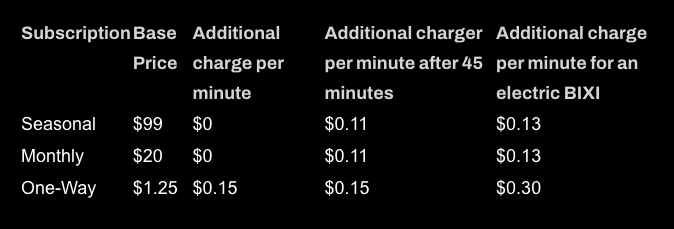
\includegraphics[scale=0.40]{images/BikePrices.png}
    \caption{Subscription Charges}
    \label{fig:my_label1}
\end{figure}

\newpage
\subsection{Description}
The solution is an online web application allowing a customer to purchase a iGo bike rental pass, top up their iGo account, and obtain a code to unlock a bike from a iGo station. The iGo Vending Machine will communicate with iGo system over an appropriate communication link.\\

A user will be required to sign up for an account with the iGo Vending Machine on their first visit. In order to purchase a pass or top up their account, a user is required to link their iGo account with their iGo Vending Machine account. After signing up successfully, a user will be able to proceed with one or more transactions. Their iGo account will be linked to their iGo Vending Machine account and hence will be linked to all transactions made under their iGo Vending Machine account. A user will be able to use their existing iGo account to rent a bike from any iGo station.\\



The iGo Vending Machine must be able to provide the following services to iGo users:
\begin{enumerate}
    \item A user must be able to sign up for a iGo Vending Machine account online, with their email address and be able to link their iGo account to their iGo Vending Machine account.
    \item A user must be able to purchase a iGo bike rental pass, selecting from different types of passes, such as daily or monthly passes. The transaction could be made via Visa or Mastercard, or Paypal.
    \item A user must be able to top up their iGo account balance to rent bikes.
    \item A user must be able to view their existing iGo account balance.
    \item A user must be able to view their iGo rental history and must be able to print out their rental history.
    \item A user must be able to schedule their rental pass for a future date.
    \item A user must be able to obtain a code to unlock a bike from a iGo station after making a successful transaction. The code must be valid for a limited time.
    \item A user must be able to unlink any iGo accounts under their iGo Vending Machine account.
\end{enumerate}

\begin{figure}[H]
    \centering
    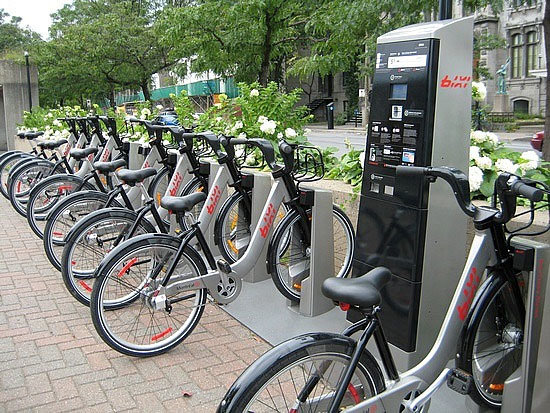
\includegraphics[scale=0.40]{images/BixiStation.png}
    \caption{Drop off station for bikes}
\end{figure}



The iGo Vending Machine will communicate each transaction to the iGo system and obtain verification that the transaction was successful. The iGo Vending Machine will connect with the iGo system to make sure transactions are successfully made.\\
If iGo determines that the email exists in their database, a user will be required to log in or use another email to register. If iGo determines that the iGo account is linked to another existing iGo Vending Machine account, a user will not be able to link this iGo account to their iGo Vending Machine account unless that iGo Vending Machine account unlinks this iGo account on the iGo Vending Machine. In all cases, the iGo Vending Machine is required to display an explanation of the problem.\\
The iGo Vending Machine will also maintain its internal log of transactions to facilitate resolving ambiguities arising from a connection failure in the middle of transactions between the iGo Vending Machine and the iGo system. Entries will be made in the log when a user registers an account, logs in and is working on their login session.



\subsection{Project Assumption}
For this project, it is assumed that the iGo bike sharing service will provide a secure and reliable application programming interface (API) for the online ticket vending machine to access and update ticket information, such as ticket availability and pricing. It is also assumed that the iGo system will be able to receive and process online ticket purchases made through the vending machine, and update the system with the appropriate information, such as the rental duration and the number of available bikes. Additionally, it is assumed that the online ticket vending machine will be integrated with a secure payment gateway that is capable of handling online transactions securely and efficiently.\\
These assumptions are necessary for the successful development and implementation of the online ticket vending machine for iGo bike sharing service.

%%%%%%%%%%%%%%%%%%%%%%%%%%%%%%%%%%%%%%%%%%%%%%%%

\section{PROBLEM 2}
\subsection{Problem Domain Model}
\subsubsection{Class Diagram}
\begin{figure}[H]
    \centering
    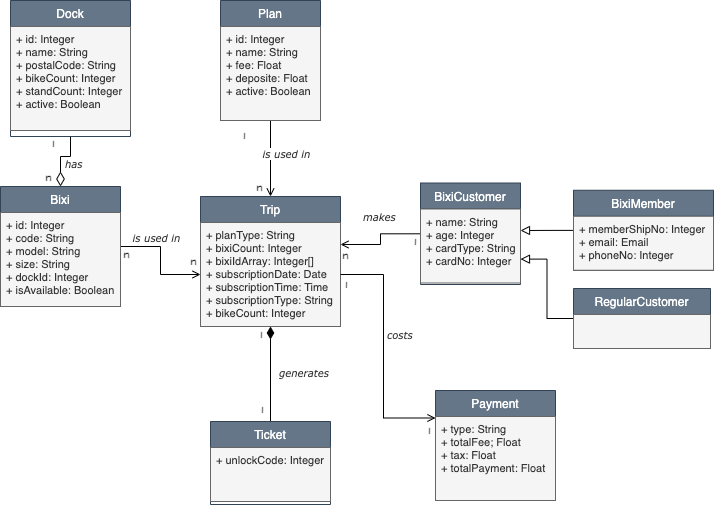
\includegraphics[scale=0.70]{images/ClassDiagram.png}
    \caption{UML Class Diagram}
\end{figure}
Shown above are the class and package diagrams for iGo.

The domain model of our iGo system, bike-sharing system, is represented by several classes and relationships between classes.\\

The Trip class is the main class of the iGo system. It keeps the information of biking trips, including bike count, start date and time, bike type, customer and other parameters. This information is essential for renting a bike and will be updated after returning the bike.\\

We have two types of customers, the regular one which rents bikes for one-path trips or who has a membership in the iGo system based on different plans. We have extra attributes in the member class to keep the contact information and membership number. They have common characteristics, such as name or age and card info as a parent class. The condition and features of different plans selected by customers are shown as plan class.\\

The iGo class refers to attributes of bikes in the iGo system. The model of bike (regular or electrical), size, dock id and its availability are examples of attributes of this class.\\

The information of dockes through the city and number of bikes they have are considered as Dock class.\\

The system also includes other classes such as the ticket class that generates a ticket with unlock code. The unlock code is a temporary one to unlock the bike situated in the dock by the customer to start the journey.\\

The Payment class represents the information of payment in different steps of the trip, including renting and returning based on the plan, customer type and time ride by customer.\\
\subsubsection{Package Diagram}

\begin{figure}[H]
    \centering
    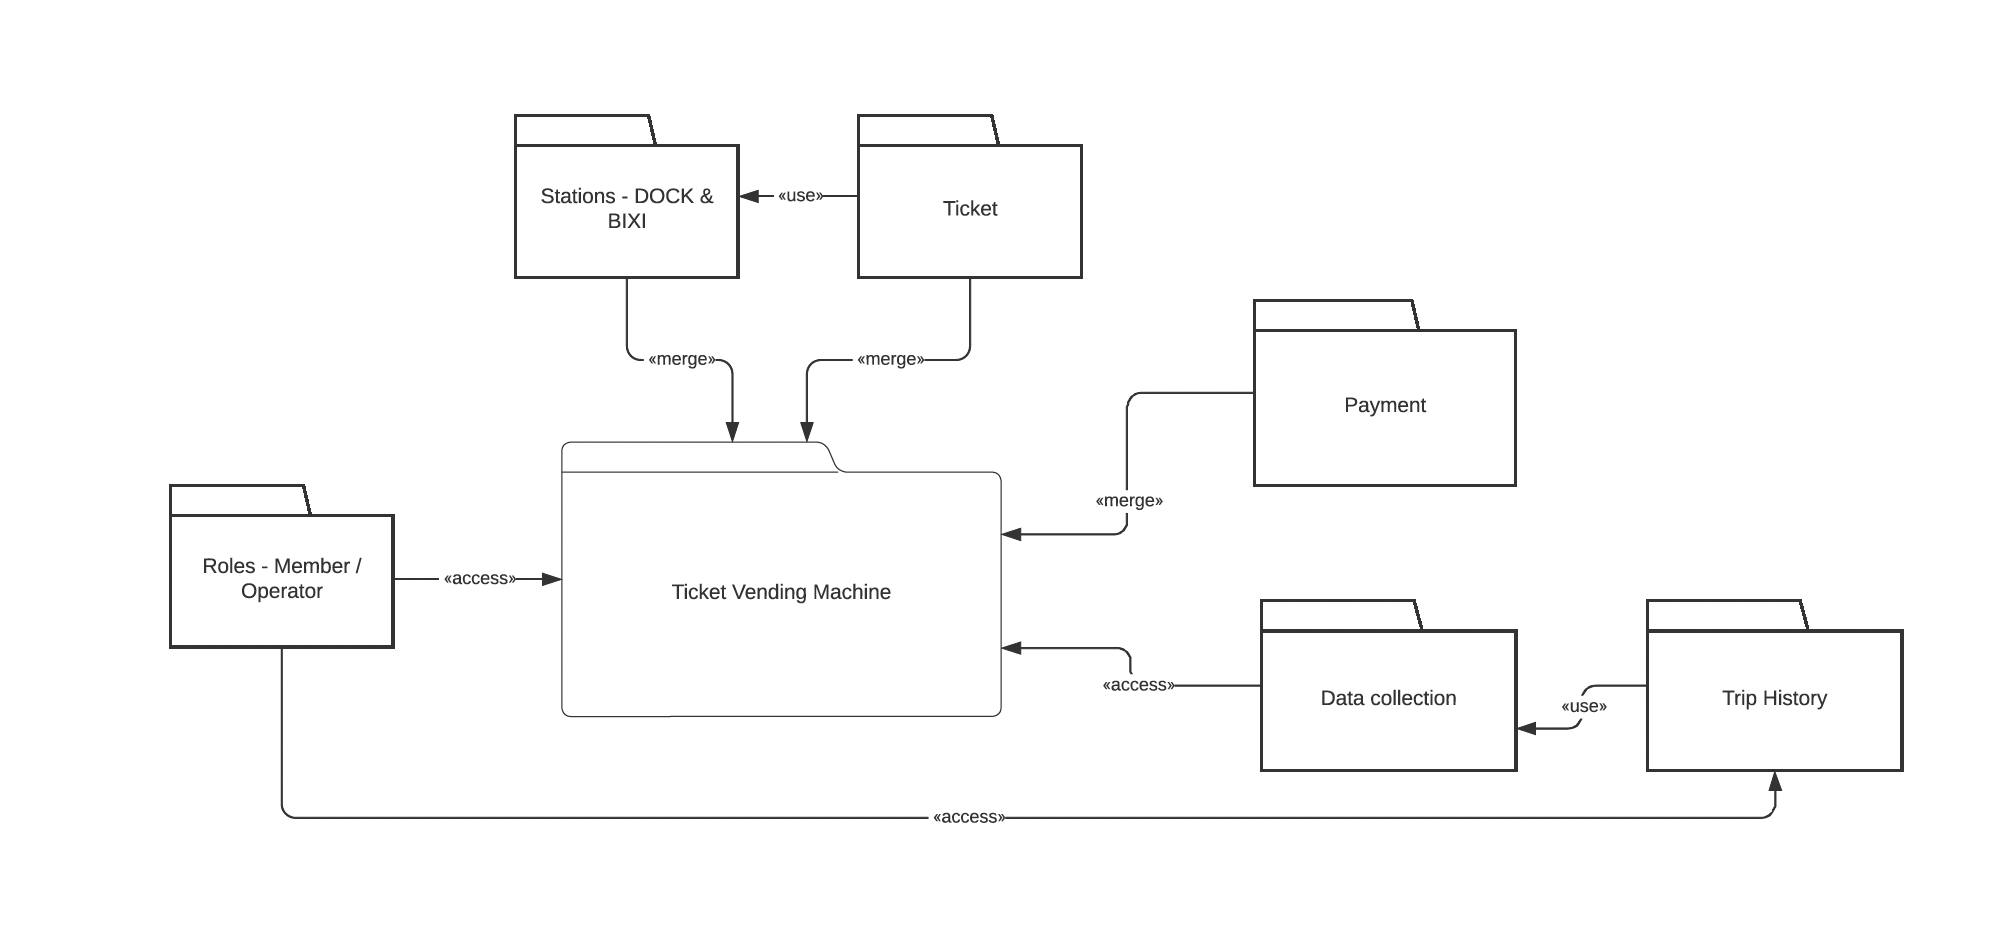
\includegraphics[scale=0.40]{images/UMLPackageDiagram.png}
    \caption{UML Package Diagram}
\end{figure}

The above diagram shows the packages for iGo system that connects the bike system to the TVM. The application also stores the trip history of each user that collects the user data and uses to link the trip to the user.


%%%%%%%%%%%%%%%%%%%%%%%%%%%%%%%%%%%%%%%%%%%%%%%%
\section{PROBLEM 3}
\subsection{Mind Map}
A mind map that illustrates the relationships that exist between various components of the whole idea.

By brainstorming with our team on the different elements of the interview process, we identified the following key aspects / elements that we needed to consider – 
\begin{enumerate}
    \item Participants
    \begin{itemize}
        \item Interviewers - We needed to identify the people who could give us correct answers to our questions which required locating actual users of the iGo service which was to be our template for the iGO project. We were mindful of the fact that a customer who uses the service frequently would be able to reply with more details than a user who has only used iGo occasionally.
        \item Interviewees – We took special care to make sure that the person giving the interview knew the interviewer and shared an ease of comfort in conversations with them to make the interview process comfortable for the interviewee.
    \end{itemize} 
    \item Medium – We also thought carefully about which medium we should conduct our interviews. Most of our decisions were taken to facilitate ease and comfort of the interviewees. So we chose to conduct it Online when they did not live nearby the interviewers. Since interviewees could feel added burden of appearing good on camera, we chose to conduct the interview only in the audio format. We also provided the interviewees with an early draft of our question sets to let them think of their answers beforehand.
    \item Interview Perspective -  We also considered the different point of views we could take to ask our question. Within the User Perspective, interviewer will focus on questions about the user’s experience using the service in his life and how the service helped him in his life. The maintenance perspective is for the engineers of the systems working to keep the TVM error free to provide the best service. Risk analysis perspective dealt with questions related to finding out user actions that could harm the system like theft and accidents. Update and Extensibility perspective is for engineers working to add new services to the system to let them know which services are most asked for by the interviewees.
    \item Question Topics – In this section we brainstormed over what different areas of the system we needed information for. Guided by these topics, we created our question. The second mindmap of this submission shows the breakdown of questions we brainstormed and researched either through interviews or external sources.
    \item Information Sources – TO enhance the results of the information gathering phase through interviews, we took aid from other sources both to help identifying areas we were unfamiliar and needed interview for and also to crosscheck and validate the information given by the interviewers. BIXI’s official site ‘https://bixi.com/en/bixi-inc’ was of great help. We also went over reddit posts by BIXI customers to learn of their experiences with the BIXI system. We also found other posts on some travel review sites to add to our understanding of the system.\cite{MindMap}
\end{enumerate}	

\begin{figure}[H]
    \centering
    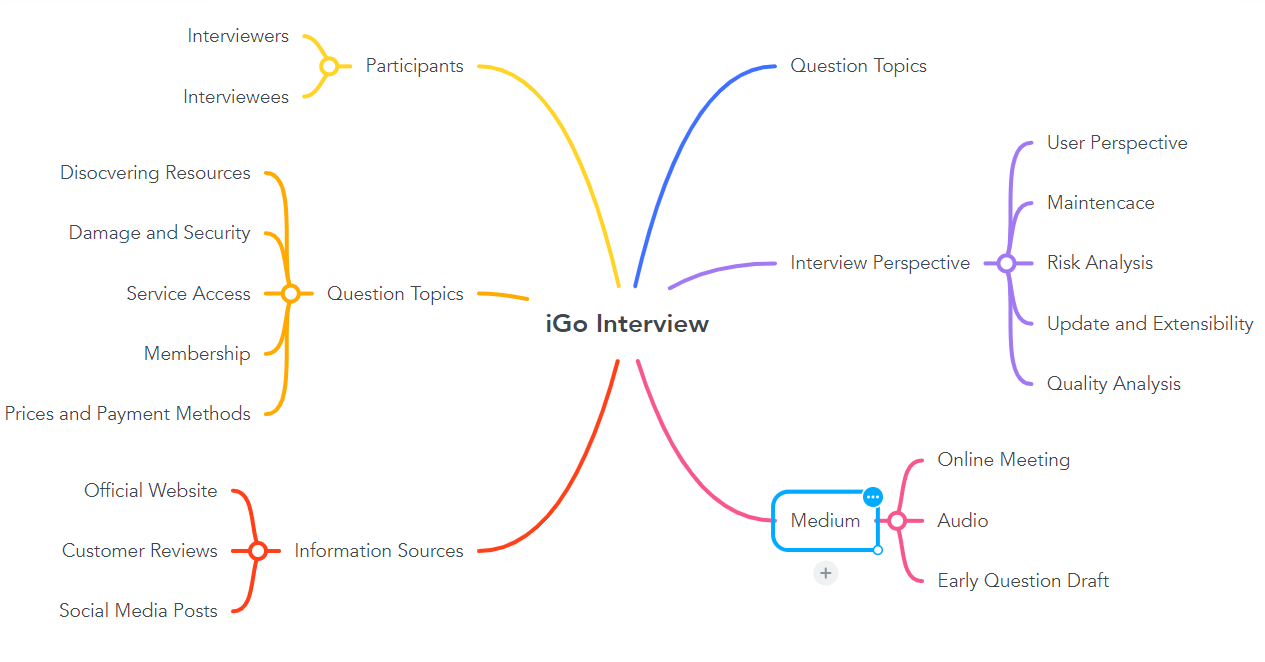
\includegraphics[scale=0.60]{images/MindMapElements.png}
    \caption{Mind Map Elements}
\end{figure}

\newpage
\subsection{Mind Map Interviews}
The mind map interviews are conducted and the recording of each interview has been linked on the github repository. The transcription of each interview has been documented in the \nameref{Appendix} section of the document.

\begin{figure}[H]
    \includegraphics[width=0.9\linewidth,height=10cm]{images/MindMapInterviews.png}
    \caption{Mind Map Interview Elements}
\end{figure}

%%%%%%%%%%%%%%%%%%%%%%%%%%%%%%%%%%%%%%%%%%%%%%%%
\section{PROBLEM 4}
\subsection{Use Case Models - Spatial Relationship}
A use case model here describes the proposed functionality of the system in terms of Users, iGo and Bank actors. It is the visual representation of system's behaviour that defines interactions between the system, Users and other actors. The use case model shows the relationship between use cases and actors.\cite{Unlock}

\subsubsection{Rent Bike}
\begin{table}[H]
\begin{center}
\renewcommand{\arraystretch}{2}
\begin{tabular}{|p{8cm}|p{8cm}| } 
 \hline
 \textbf{NAME} & Rent bike\\ 
 \hline
 \textbf{ID} & UC1  \\ 
 \hline
 \textbf{ACTORS} & User\\ 
 \hline
 \textbf{DESCRIPTION} & The User initiates renting a bike by selecting the number of trips or by renewing their old membership \\ 
 \hline
 \textbf{NORMAL FLOW} & \begin{enumerate}
     \item The user selects the language
     \item Inserts the payment card for validation
     \item Chooses no of trips
     \item Proceeds to payment
 \end{enumerate} \\
 \hline
 \textbf{PRE-CONDITIONS} & User starts the interaction with the TVM\\
 \hline
 \textbf{POST-CONDITION} & User ends at payment for the no of trips selected\\
 \hline
 \textbf{EXCEPTIONS} & The user cancels the session\\
 \hline
\end{tabular}
\caption{\label{demo-table}Use Case 1 - Rent bike use case description}
\end{center}
\end{table}

\subsubsection{Validate Card}
\begin{table}[H]
\begin{center}
\renewcommand{\arraystretch}{2}
\begin{tabular}{|p{8cm}|p{8cm}| } 
 \hline
 \textbf{NAME} & Validate card\\ 
 \hline
 \textbf{ID} & UC2  \\ 
 \hline
 \textbf{ACTORS} & User, Bank\\ 
 \hline
 \textbf{DESCRIPTION} & The user inserts the payment card to initiate the process for renting a bike \\ 
 \hline
 \textbf{NORMAL FLOW} & \begin{enumerate}
     \item The user selects the language
     \item Inserts the payment card for validation
 \end{enumerate} \\
 \hline
 \textbf{PRE-CONDITIONS} & User initiates renting a bike by selecting language\\
 \hline
 \textbf{POST-CONDITION} & User chooses no of trips after validating card\\
 \hline
 \textbf{EXCEPTIONS} & The user cancels the session\\
 \hline
\end{tabular}
\caption{\label{demo-table}Use Case 2 - Validate customer card case description}
\end{center}
\end{table}


\subsubsection{Make Payment}
\begin{table}[H]
\begin{center}
\renewcommand{\arraystretch}{2}
\begin{tabular}{|p{8cm}|p{8cm}| } 
 \hline
 \textbf{NAME} & Payment\\ 
 \hline
 \textbf{ID} & UC3  \\ 
 \hline
 \textbf{ACTORS} & User, Bank, TVM\\
 \hline
 \textbf{DESCRIPTION} & A payment receipt is produced after a successful transaction \\  
 \hline
 \textbf{NORMAL FLOW} & \begin{enumerate}
     \item The user selects the language
     \item Inserts the payment card for validation
 \end{enumerate} \\
 \hline
 \textbf{PRE-CONDITIONS} & User initiates the payment after selecting no of trips\\
 \hline
 \textbf{POST-CONDITION} & User generates the payment/bike receipt\\
 \hline
 \textbf{EXCEPTIONS} & The payment fails\\
 \hline
\end{tabular}
\caption{\label{demo-table}Use Case 3 - Payment case description}
\end{center}
\end{table}

\subsubsection{Generate Ticket}
\begin{table}[H]
\begin{center}
\renewcommand{\arraystretch}{2}
\begin{tabular}{|p{8cm}|p{8cm}| } 
 \hline
 \textbf{NAME} & Generate Ticket\\ 
 \hline
 \textbf{ID} & UC4  \\ 
 \hline
 \textbf{ACTORS} & User\\
 \hline
 \textbf{DESCRIPTION} & The user can select the mode of the receipt either via email or SMS or by printing it \\  
 \hline
 \textbf{NORMAL FLOW} & \begin{enumerate}
     \item The user chooses the mode of receipt retrieval
     \item If email or SMS mode selected user enters email address or phone number respectively
 \end{enumerate} \\
 \hline
 \textbf{PRE-CONDITIONS} & After successful payment user chooses mode of receipt retrieval\\
 \hline
 \textbf{POST-CONDITION} & User unlocks the bike with the code provided in the receipt\\
 \hline
 \textbf{EXCEPTIONS} & Either email address or phone number is invalid\\
 \hline
\end{tabular}
\caption{\label{demo-table}Use Case 4 - Generate Ticket case description}
\end{center}
\end{table}

\subsubsection{Return Bike}
\begin{table}[H]
\begin{center}
\renewcommand{\arraystretch}{2}
\begin{tabular}{|p{8cm}|p{8cm}| } 
 \hline
 \textbf{NAME} & Return bike\\ 
 \hline
 \textbf{ID} & UC5\\ 
 \hline
 \textbf{ACTORS} & User\\
 \hline
 \textbf{DESCRIPTION} & After trip completion user's trip info is updated by TVM and proceeds to return bike procedure \\  
 \hline
 \textbf{NORMAL FLOW} & \begin{enumerate}
     \item User inserts the payment card for validation
     \item The TVM updates user's trip info with per min cost and displays the final cost
     \item User pays for the calculated cost
 \end{enumerate} \\
 \hline
 \textbf{PRE-CONDITIONS} & User checks for the dock that has an empty spot\\
 \hline
 \textbf{POST-CONDITION} & User initiates the payment after the trip info update\\
 \hline
 \textbf{EXCEPTIONS} & \\
 \hline
\end{tabular}
\caption{\label{demo-table}Use Case 5 - Return bike case description}
\end{center}
\end{table}

\subsubsection{Update Trip}
\begin{table}[H]
\begin{center}
\renewcommand{\arraystretch}{2}
\begin{tabular}{|p{8cm}|p{8cm}| } 
 \hline
 \textbf{NAME} & Update trip info\\ 
 \hline
 \textbf{ID} & UC6\\ 
 \hline
 \textbf{ACTORS} & TVM\\
 \hline
 \textbf{DESCRIPTION} & After trip completion user finds a dock with empty spot and inserts payment card for trip updation \\  
 \hline
 \textbf{NORMAL FLOW} & \begin{enumerate}
     \item User inserts payment card and validates it to begin the return process
     \item The TVM updates user's trip info with per min cost and displays the final cost
 \end{enumerate} \\
 \hline
 \textbf{PRE-CONDITIONS} & User checks for the dock that has an empty spot\\
 \hline
 \textbf{POST-CONDITION} & User initiates the payment after the trip info update\\
 \hline
 \textbf{EXCEPTIONS} & N/A\\
 \hline
\end{tabular}
\caption{\label{demo-table}Use Case 6 - Update trip info case description}
\end{center}
\end{table}

\subsection{Use case Model Diagrams}
\subsubsection{Renting a bike}
\begin{figure}[H]
  \centering
  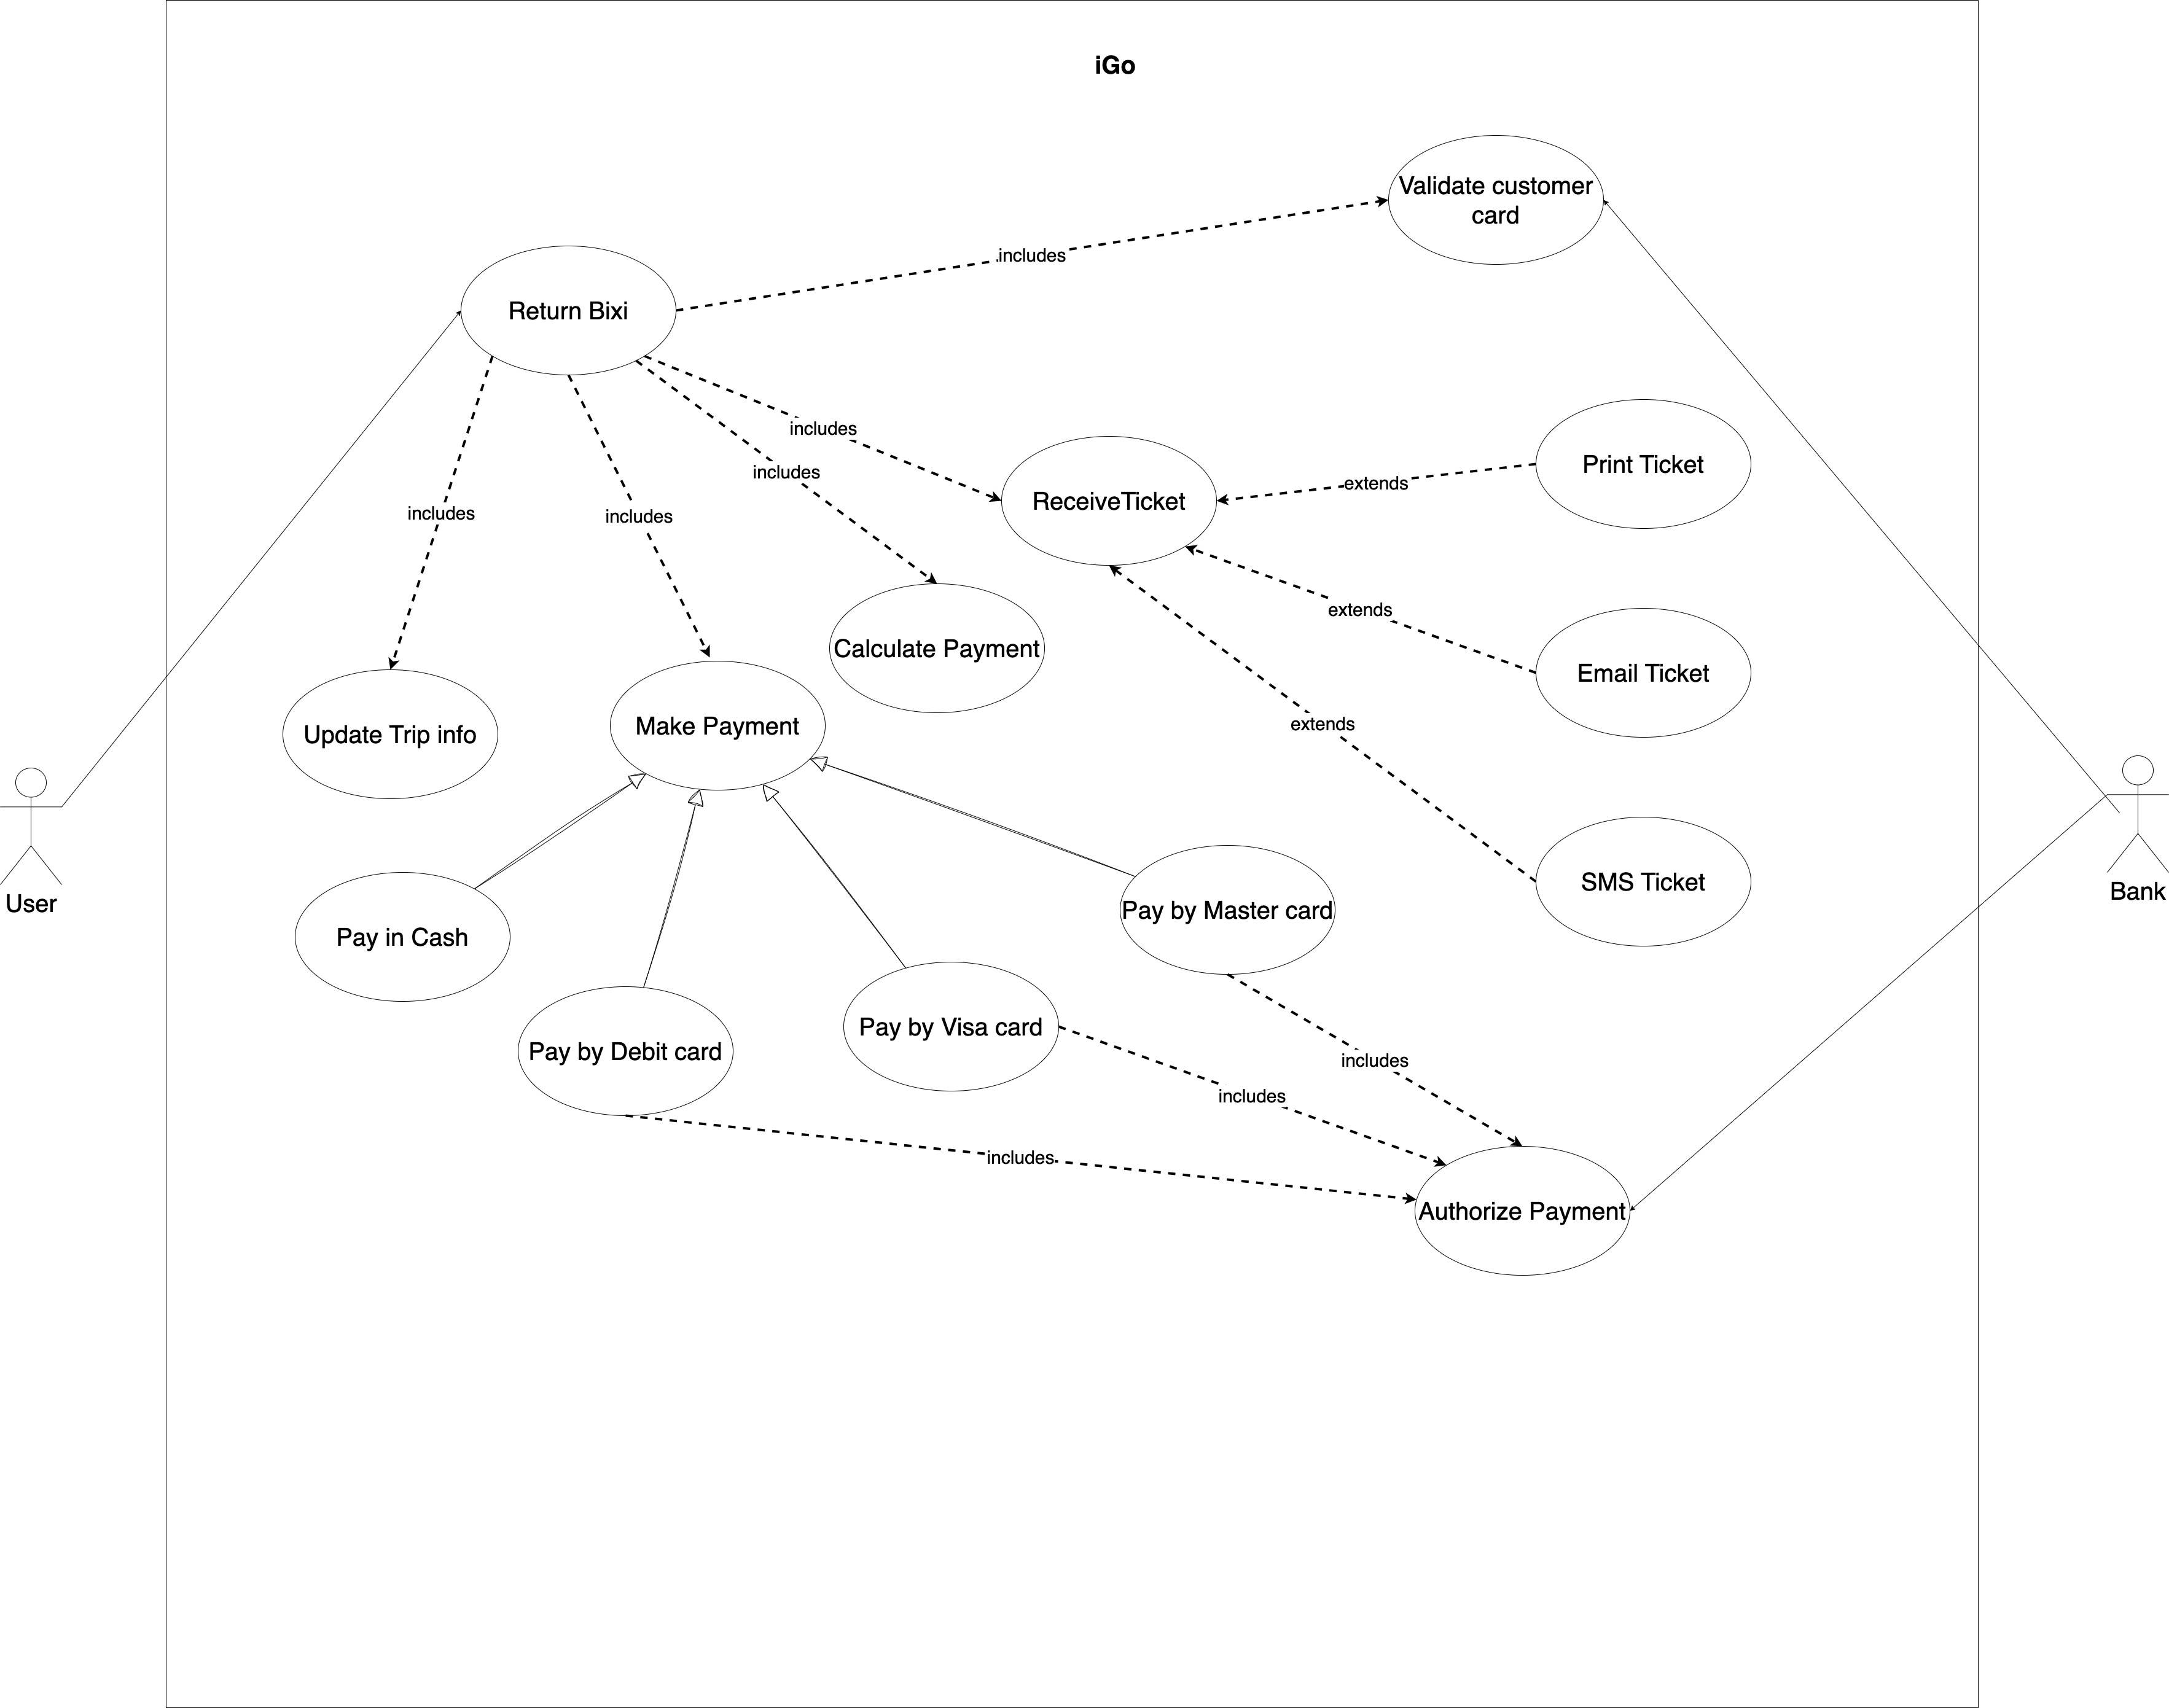
\includegraphics[width=17cm, height=12cm]{images/rentBixiUseCase.jpg}
  \caption{Rent bike Use Case Model Diagram}
  \label{fig:Rent bixi Case Model Diagram}
\end{figure}

\subsubsection{Returning a bike}
\begin{figure}[H]
  \centering
  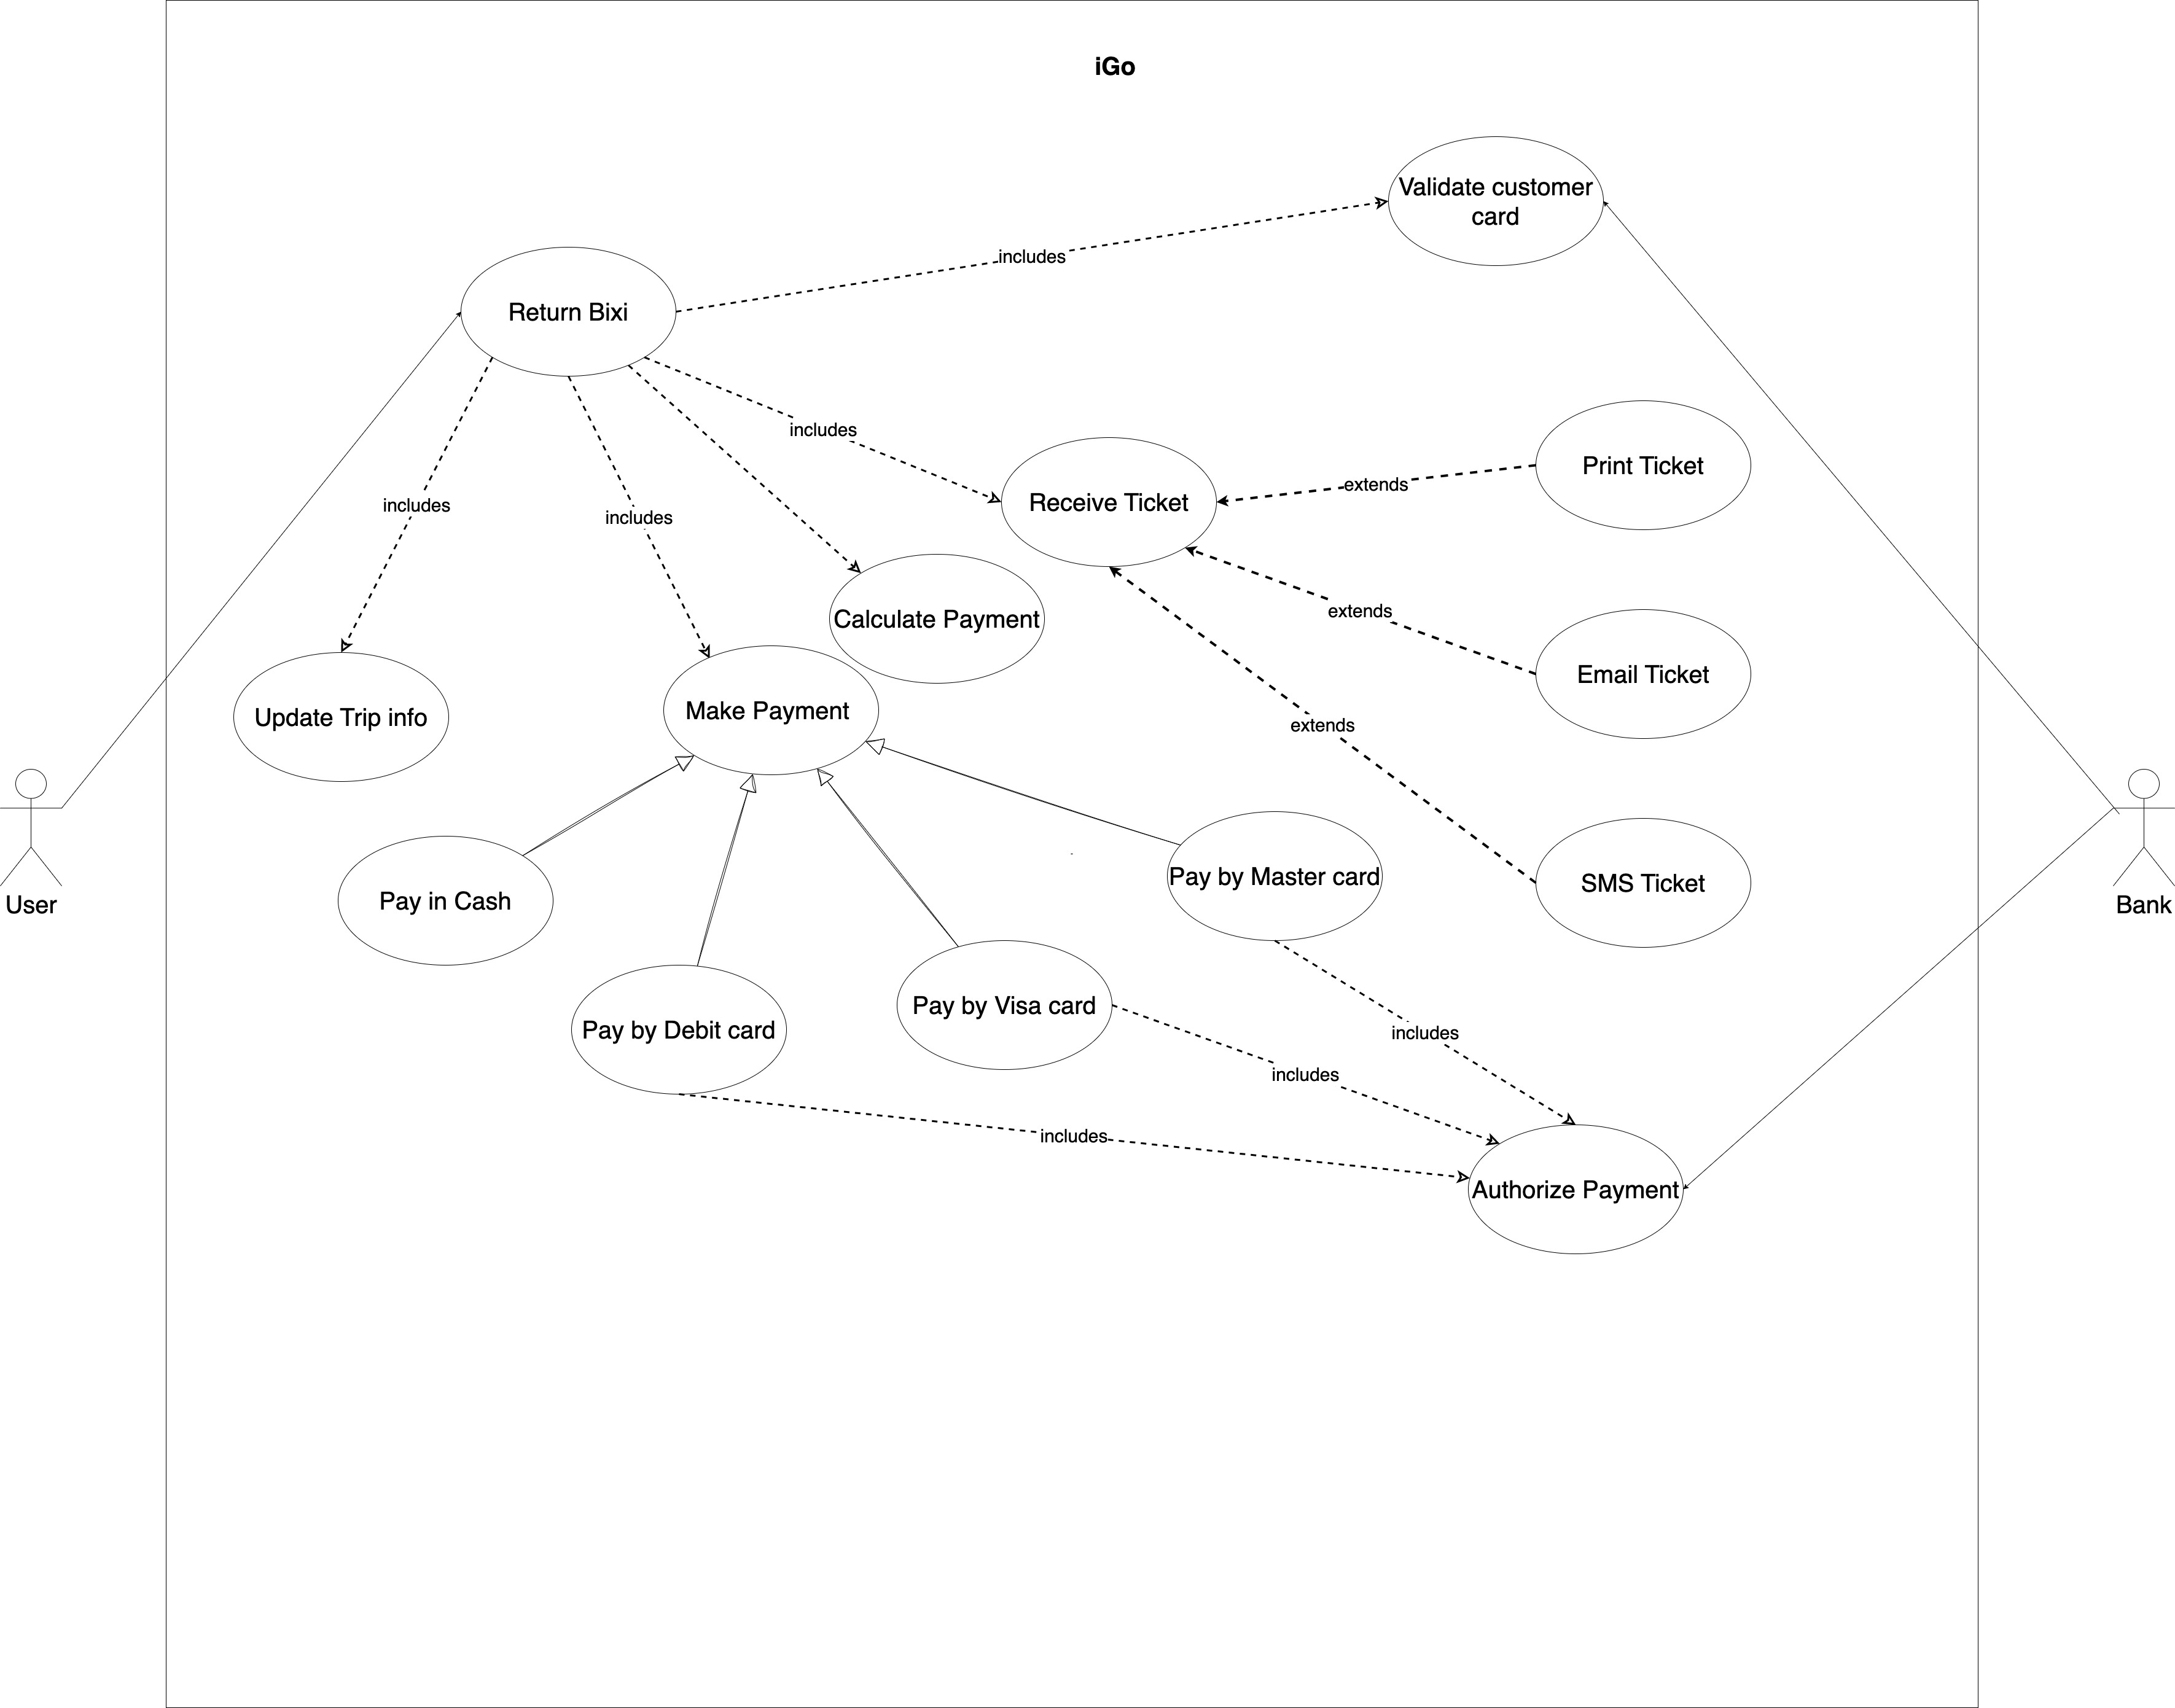
\includegraphics[width=17cm, height=12cm]{images/returnBixiUseCase.jpg}
  \caption{Return bike Use Case Model Diagram}
  \label{fig:Return bixi Case Model Diagram}
\end{figure}

%%%%%%%%%%%%%%%%%%%%%%%%%%%%%%%%%%%%%%%%%%%%%%%%
\newpage
\section{PROBLEM 5}
\subsection{Use Case Diagram - Temporal Relationship}
In order to analyze the temporal relationships between the critical use cases and the order in which the steps are perform in a use case, we have constructed UML activity diagrams to visualize the details.
\subsubsection{Signing up}
This use case model indicates the steps to sign up an account via the application.
\begin{figure}[H]
  \centering
  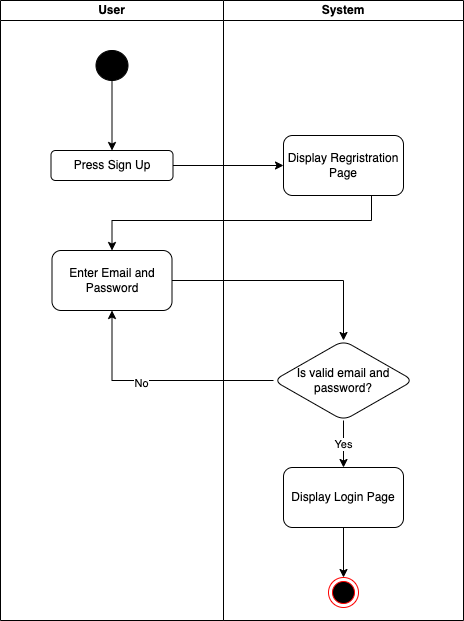
\includegraphics[scale = 0.60]{images/SignUpActivity.png}
  \caption{Sign Up Activity Diagram}
  \label{fig:Sign Up Activity Diagram}
\end{figure}
\newpage
\subsubsection{Finding the station}
This use case diagram shows how to find the station for returning the bike.
\begin{figure}[H]
  \centering
  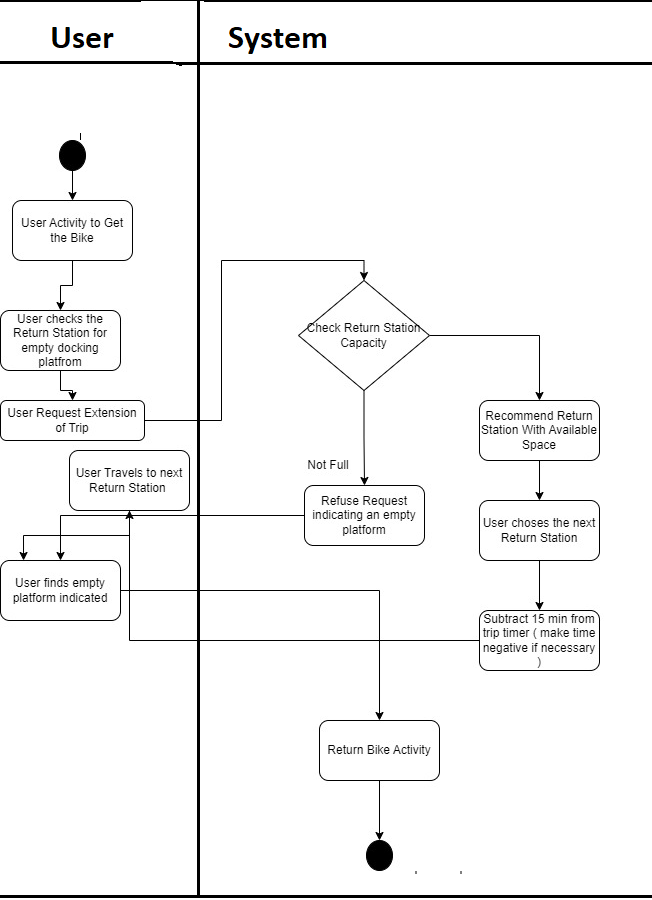
\includegraphics[scale = 0.70]{images/UserActivityfindingStation.png}
  \caption{Finding a dock station}
  \label{fig:finding_station}
\end{figure}
\newpage
\subsubsection{Purchasing a ticket}
The use case models below illustrate the details in the scenario of purchasing a ticket (one is via app, the other is at kiosk) and the temporal relationships between the use case of renting a bike and the use case of making a payment.
\begin{figure}[H]
  \centering
  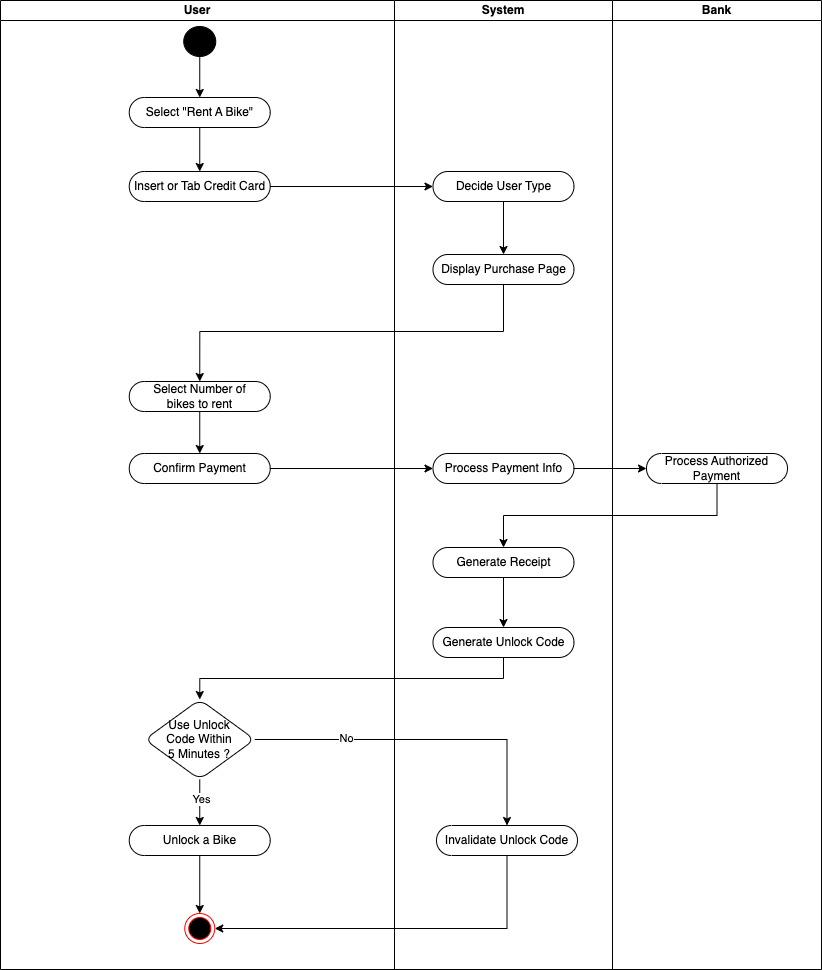
\includegraphics[scale = 0.50]{images/PurchaseTicketAtKiosk.png}
  \caption{Purchase a Ticket at Kiosk Activity Diagram}
  \label{fig:Purchase a Ticket at Kiosk Activity Diagram}
\end{figure}
\begin{figure}[H]
  \centering
  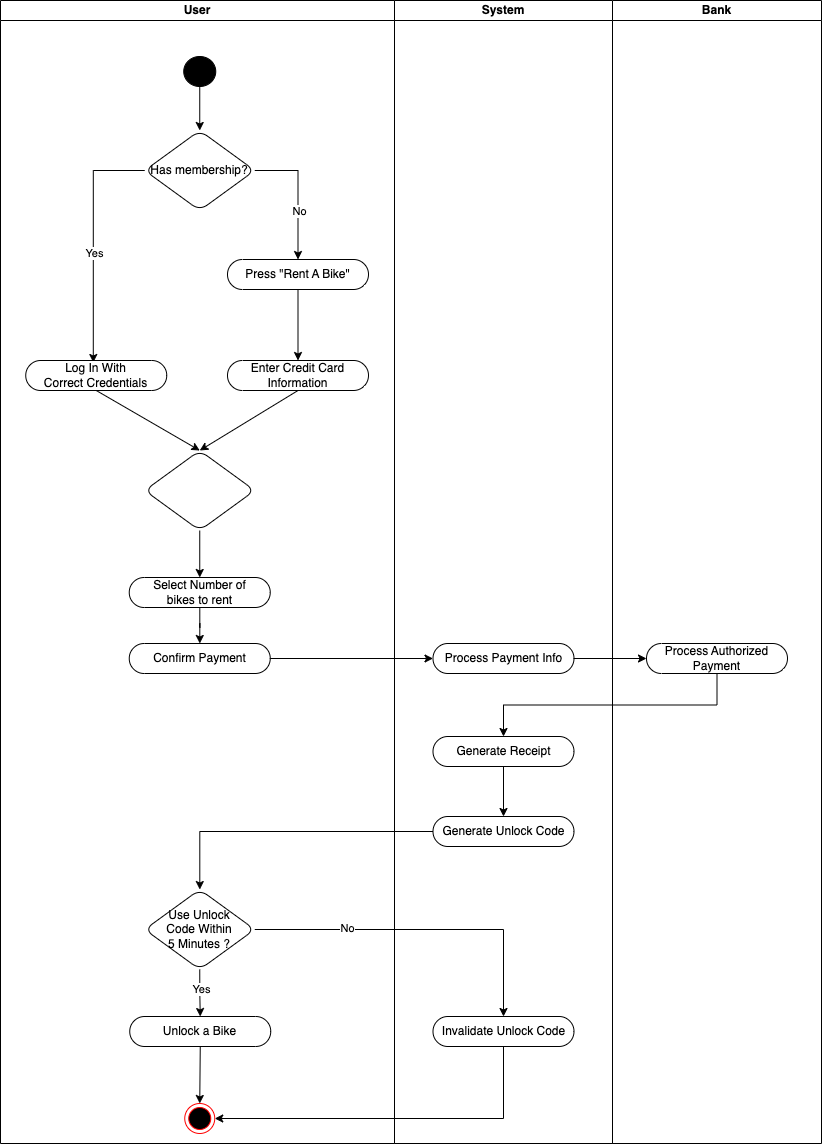
\includegraphics[scale = 0.60]{images/PurchaseTicketViaApp.png}
  \caption{Purchase a Ticket via App Activity Diagram}
  \label{fig:Purchase a Ticket via app Activity Diagram}
\end{figure}

\subsubsection{Returning a bike}
This use case activity model shows the steps to return a bike at the docking station.
\begin{figure}[H]
  \centering
  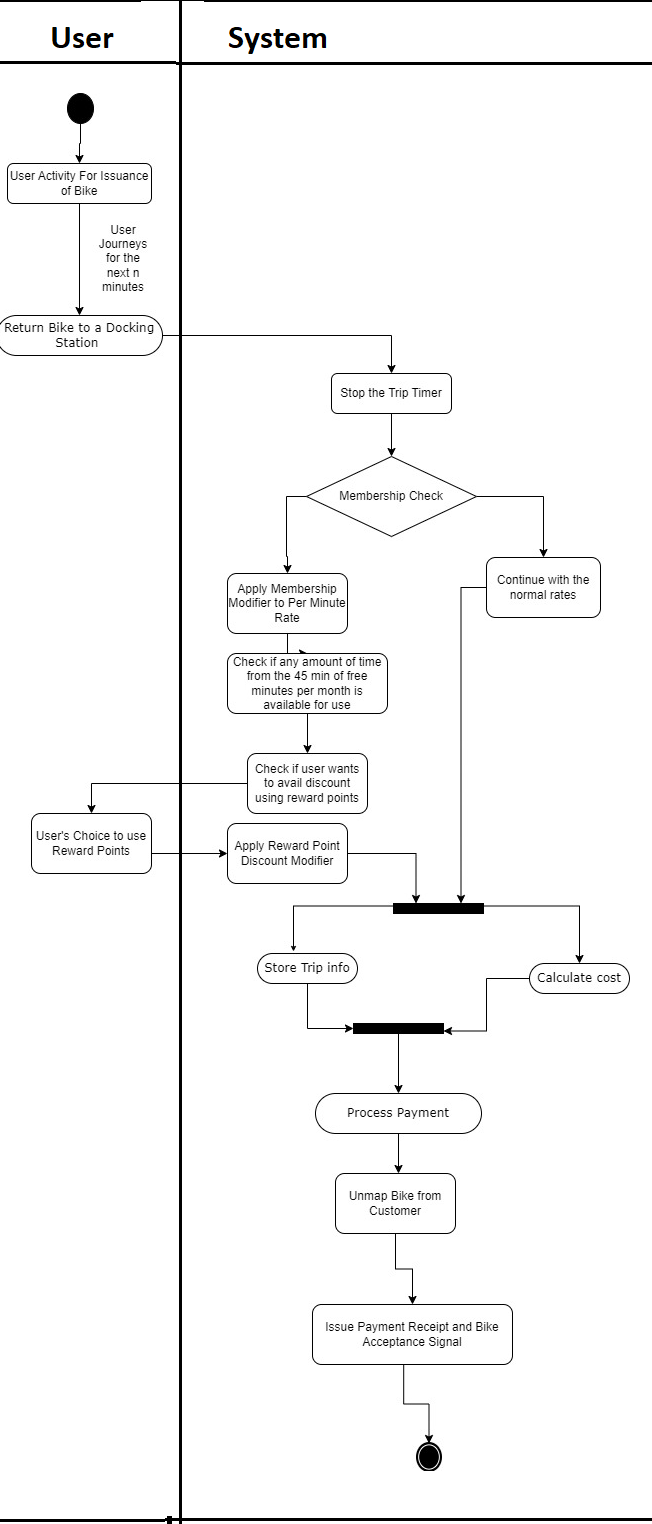
\includegraphics[scale = 0.60]{images/UserActivityDiagramReturnBike.png}
  \caption{User activity for returning a bike}
  \label{fig:return_bike}
\end{figure}


\subsubsection{Award Points}
This use case model shows the award points that the user obtains once he rents and returns a bike.
\begin{figure}[H]
  \centering
  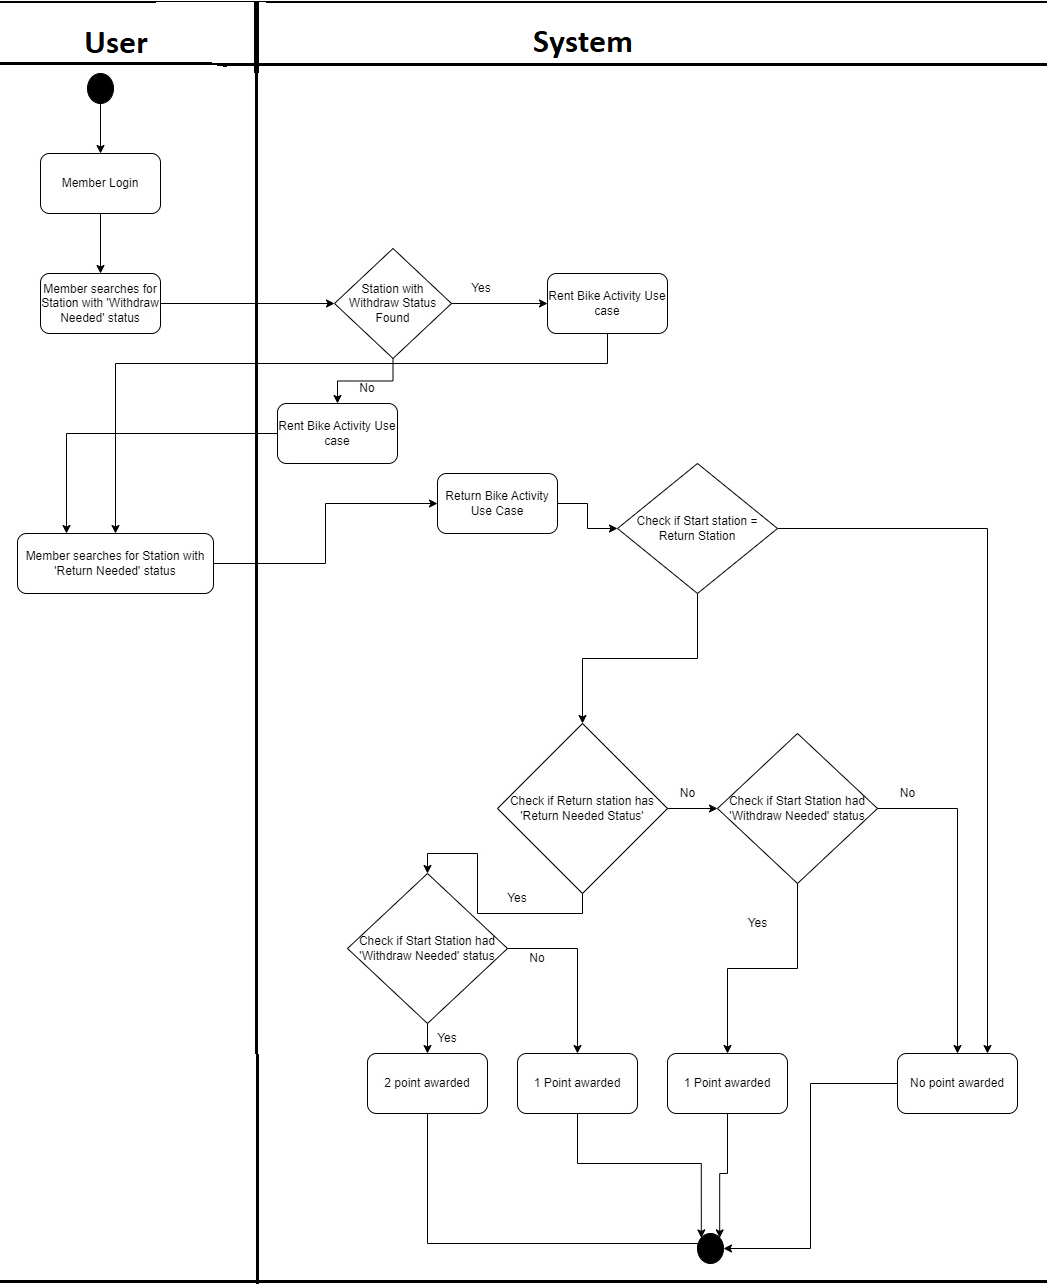
\includegraphics[scale = 0.60]{images/AwardPointsActivityDiagram.png}
  \caption{Earning award points}
  \label{fig:Earning_awards}
\end{figure}

\newpage
\subsubsection{Purchasing a membership}
This activity model shows the scenario of purchasing a membership from the application.
\begin{figure}[H]
  \centering
  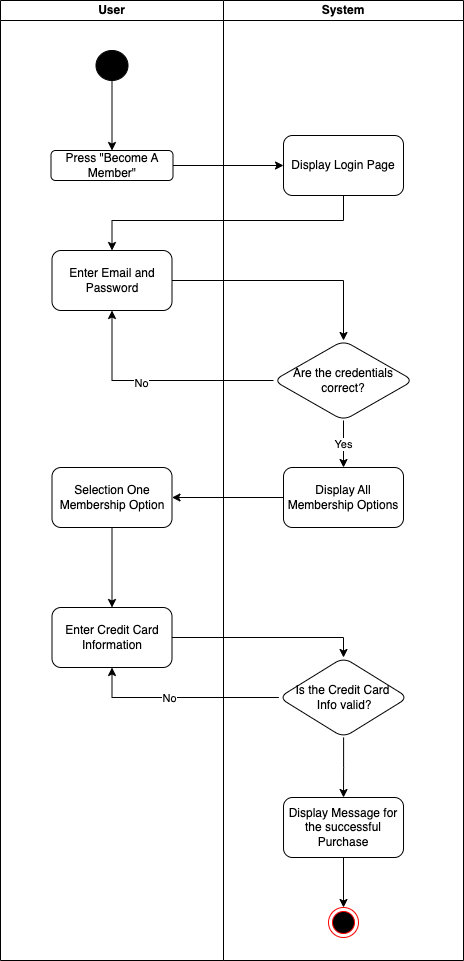
\includegraphics[scale = 0.55]{images/PurchaseMembershipActivity.png}
  \caption{Purchase Membership Activity Diagram}
  \label{fig:Purchase Membership Activity Diagram}
\end{figure}







\chapter{Conclusion}
The significant outcome of this object-oriented software engineering project is that it allowed us to learn how to work as a team, coordinate together, apply industry standards, and follow continuous integration/ continuous development using agile and rigid methodologies.\\
iGo as an object-oriented software for public bike transportation helps people with renewing, managing, and purchasing subscription services for bike transportation with user-friendly and professional options.  This report provides an overview of the iGo services showcasing the problem domain model, UML package diagram used to organize the elements, mind map which focuses on the elements for the interview process and use case model for iGo showing the spatial relationship.\\
In conclusion, the report presents a collection of interconnected artifacts that address the problem domain as well as the solution domain for the software component of a TVM that is usable, maintainable, secure, and sustainable.

%%%%%%%%%%%%%%%%%%%%%%%%%%%%%%%%%%%%%%%%%%%%%%%
\appendix
\chapter{Appendix}\label{Appendix}
\section{Interview 1}
\begin{enumerate}
    \item Rishab Kumar - What happens if the Bixi dock is full?
    \newline User - We can request for a 15 mins time credit free of charge so that we may return it to some other nearby BIXI station
    \item Naman Kumar - Why would you want to rent an e-bike over a traditional bike?
    \newline User - Its easy to ride than traditional bikes ,Also I can cover larger distance over short period of time. Also , there is less physical exertion at the end of day. 
    \item Rishab Kumar - But its more costlier than traditional bikes ?
    \newline User - Yes , but it saves a lot of time , I also work as a part time food delivery worker,so its   easier for me to commute and cover the costs.
    \item Naman Kumar - How do you know if the BIXI is fully charged?
    \newline User - there will be 4 green bars on the Bixi stem which means its fully charged.
    \item Naman Kumar - Which pass do you usually opt for BIXI?
    \newline User - I usually opt for monthly pass as I use bixi very often . 
    \item Rishab Kumar - How much does it cost?
    \newline User - It costs around 20 dollars a month . it covers unlimited rides upto 45 mins.
    \item Rishab Kumar - What about after 45 mins?
    \newline User - I think its 11 cents per min after that.
    \item Rishab Kumar - Does Bixi provides any additional discounts ?
    \newline User - Yes , For concordia students , they provide 15 percent discounts on plans. 
    \item Naman Kumar - What if the Bixi that you get is defective?
    \newline User - This usually doesnt happen , but if it happens , we can leave that one to the dock and we can press the red button on docking station to notify the technician.
\end{enumerate}







\newpage
\section{Interview 2}
\begin{enumerate}
    \item Mansi: Hi,how are you doing?
    \newline Pal: I am good, how are you?
    \item Mansi: I am good thank you, May I know you name to address you?
    \newline Pal: My name is Pal sheth.
    \item Mansi: okay, hello Pal so do I have the permission to audio record you for the feedback interview of the TVM?
    \newline Pal: Yes ofcourse
    \item Mansi: Have you interacted with the TVM to buy one time passes or purchase memberships?
    \newline Pal: Yes
    \item Mansi: How often do you travel using BIXI?
    \newline Pal: Yes I use it mostly in summers twice or thrice a week to travel within 3KM range 
    \item Mansi: How often do you use the TVM for purchasing a membership/ticket?
    \newline Pal: Mostly once a month I purchase a membership 
    \item Mansi: Do you find the TVM user friendly to get all the information you need to purchase a ticket/membership?
    \newline Pal: Yes it shows me all the information related to monthly memberships and per trip costs and I would say it is a simple process of payment and accessing a bixi using access code
    \item Mansi: Does the TVM provides you the information in the language you can read?
    \newline Pal: Yes, I can read English and it does provide information in English and French
    \item Mansi: Do you think any additional information can be shown in the TVM to make the process easy?
    \newline Pal: yes I think displaying the nearest dock where the bike I need is available is an important feature you could add in case the bike is not available in current dock. This helps in case the person buying the ticket does not have access to phone.
    \item Mansi: What can be improved to ease the process of purchasing the ticket/membership?
    \newline Pal: You can create a demo video to use the system in case of people who are unfamiliar with systems like TVM
    \item Mansi: Do you think there are enough Dock/TVM in the city to purchase the ticket?
    \newline Pal: Yes I think there are a lot in my area as I live in downtown but in more towards suburbs there are very few docks, in that case providing online option would help a lot
    \item Mansi: How would you like to get the receipt of payment?
    \newline Pal: I would like to get the option of e-receipt on the email linked
    \item Mansi: How easy is the payment system in the TVM?
    \newline Pal: I usually pay with Debit/Credit so it is fine for me
    \item Mansi:  On Scale of 1-10 how much would you rate the easiness for the process of purchasing a ticket/membership?
    \newline Pal: 8
    \item Mansi: Would you also like an Online ticket buying option apart from TVM?
    \newline Pal: Yes that would be a great option to have so that prebooking can help a lot in bixi’s availability.
    \item Mansi: Would you like to have seasonal tickets?
    \newline Pal: No I use Bixi on monthly basis some months I do use it some months I skip so monthly membership works for me
    \item Mansi: Is the TVM UI user friendly or do you have any suggestion to improve it?
    \newline Pal: No I have used the TVM many time and I am easily able to purchase a ticket
    \item Mansi: Do you want notifications for getting your Pass/Ticket purchase details or trips expiring?
    \newline Pal: Yes I would definitely like to have an e-receipt for the ticket/pass purchased to keep a record
    \item Mansi: Can you provide overall rating to TVM on the scale of 1-10?
    \newline Pal: 9
    \item Mansi: Can you suggest any improvements to the TVM?
    \newline Pal: Yes, I think displaying nearby docks with available bikes can help a lot
    \item Mansi: Okay Pal thank you for your feedback and providing time for giving feedback. 
\end{enumerate}



\newpage
\section{Interview 3}
\begin{enumerate}
    \item Yongtang Lu: Hi,how are you doing?
    \newline Pranesh: Thank you, am doing good. How about you guys?
    \item Yongtang Lu:  We are doing good, thanks. We just wanted permission to record you for the feedback of a ticket vending machine.
    \newline Pranesh: Yeah, sure. Please ask
    \item Saghana Mahesh Sarma: How often do you travel using BIXI?
    \newline Pranesh: Yes I am familiar with it, but I use it only in the summers or fall.
    \item Yongtang Lu - What is the format of the unlock code you are given when renting a bike?
    \newline Pranesh - It is a 5 digit code but they only have digits 1,2 and 3.
    \item Saghana Mahesh Sarma - Is there some way the system confirms that the Bike has been returned.
    \newline Pranesh - Yes, when you submit a bike, the docking platform’s light goes green indicating return is accepted. It is red if there is something wrong. Also, a message is sent on the app.
    \item Yongtang Lu - What happens if the station you are returning the bike to has no return platforms where you can park the bike?
    \newline Pranesh - You can request extra 15 minutes to go to the next station.
    \item Saghana Mahesh Sarma - What happens if a customer loses the unlock code?
    \newline Pranesh - You can use the terminal to get a new code issued.
    \item Yongtang Lu - But what if someone else finds it and uses it?
    \newline Pranesh - The unlock code works only for the first 5 minutes or so. After that, it does not work. So chances of that happening is very low.
    \item Saghana Mahesh Sarma - Have you ever used the membership of BIXI?
    \newline Pranesh - Actually, I generally use the membership as it is more cost effective?
    \item Saghana Mahesh Sarma - How so? How is membership more effective?
    \newline First 45 minutes are free if you are a member. So if your trips are less than 45 minutes, then you are only paying the membership cost. Also, I think we are charged less beyond that if we are member.
    \item Yongtang Lu - How does BIXI app help you ?
    \newline Pranesh - It has a map that shows stations with available bikes, icons for electric bikes and charge level. It also confirms when return is accepted. You can check out how much time has passed in your trip. Things like that. There is also a reward point system but I have no idea how it works.
    \item Saghana Mahesh Sarma: Okay Pal thank you for your feedback and providing time for giving feedback. 
\end{enumerate}



\newpage
\section{Interview 4}
\begin{enumerate}
    \item Nassrin Maarefi -Is there a time limit on how long I can keep my BIXI bike?
    \newline User - We are not supposed to keep the Bikes for more than 24 hours as it is for public use. We may incur penalties although I am not sure how much.
    \item Nassrin Maarefi - What is the mileage and speed you have seen while using Electric bike on full charge ?
    \newline User - The maximum speed I have gotten is 30 km although I haven’t tried further than that. I have travelled generally more than 5 kilometers on a full charge although I have never exhausted the battery . 
    \item Nassrin Maarefi - Do BIXI bikes have way to store items during ride?
    \newline User - Yes BIXI bikes have a basket attached to the front handle that lets you store items upto medium sized bags.
    \item Nassrin Maarefi - What are the security and safety rules that need to be followed ?
    \newline User - . We are supposed to wear helmets while we are riding the bike to conform with the general safety rules of Canada.
    \item Nassrin Maarefi - Is there any other restriction on who can use the BIXI bikes.
    \newline User - Although I have freely used the renting service as an adult, but I have heard you need a licence if the renter is between 14 to 17 years old.
    \item Nassrin Maarefi - Is there a way to reserve a bike beforehand?
    \newline User - No, I don’t think so. I have only seen bikes being taken from station when you need it.
    \item Nassrin Maarefi - Is there a period when the BIXI service is not available?
    \newline User - Yes, in last months of Winter when snow is on the roads. I think December, January you can’t. I am not sure about March and November.
    \item  Nassrin Maarefi - Can you rent for your friends?
    \newline User - Yes, you can rent multiple bikes. I think 4 is the limit, at least for the one time renting. 
    \item Nassrin Maarefi - Okay, Thank you so much for your feedback.
\end{enumerate}








\pagebreak
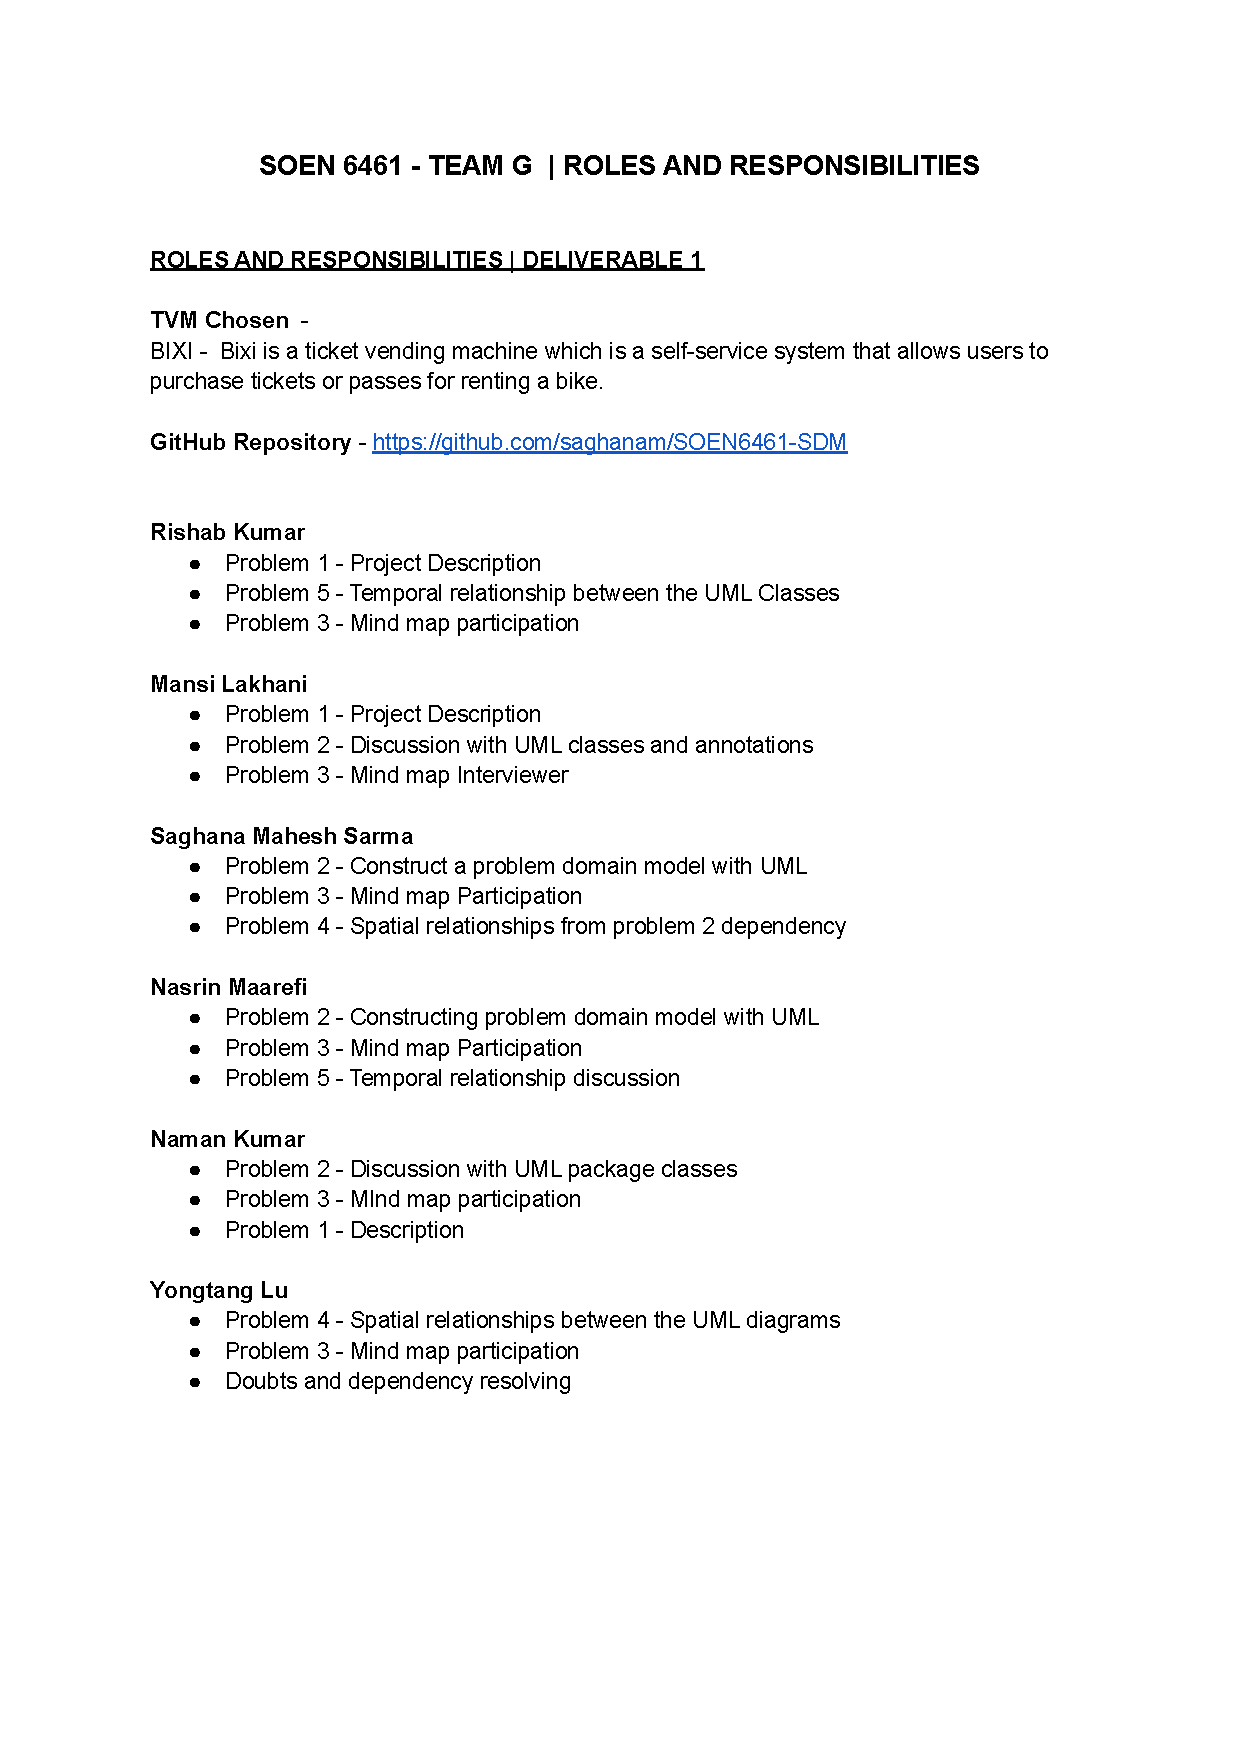
\includepdf[pages=-]{OtherFiles/RolesAndResponsibilities.pdf}
\pagebreak

\nocite{*}
\renewcommand{\bibname}{References}
\bibliographystyle{plain}
\bibliography{bibs/References.bib}

\end{document}